
%(BEGIN_QUESTION)
% Copyright 2010, Tony R. Kuphaldt, released under the Creative Commons Attribution License (v 1.0)
% This means you may do almost anything with this work of mine, so long as you give me proper credit

A globe valve with a 14 inch diameter diaphragm actuator has a bench set range of 6 to 30 PSI, which means with no process fluid pressure or friction acting on the plug, the valve will begin to open at an actuator air pressure of 6 PSI and fully open at 30 PSI:

$$\includegraphics[height=10.5cm]{i00766x01.eps}$$

Calculate the {\it seat load} force applied to the seat by the plug when there is no air pressure applied to the actuator.  Note: the ``seat load'' is a critical engineering parameter to ensure tight shut-off of the valve, especially under emergency conditions.  

Next, calculate the amount of force applied to the seat by the plug when there is 0.2758 bar of air pressure applied to the actuator:

\vskip 10pt

$F_{seat}$ @ 0 PSI = \underbar{\hskip 50pt} lb

\vskip 20pt

$F_{seat}$ @ 0.2758 bar (gauge) = \underbar{\hskip 50pt} lb

\vfil

\underbar{file i00766}
\eject
%(END_QUESTION)





%(BEGIN_ANSWER)

This is a graded question -- no answers or hints given!

%(END_ANSWER)





%(BEGIN_NOTES)

$F_{seat}$ @ 0 PSI = {\bf 923.6} lb

\vskip 10pt

$F_{seat}$ @ 0.2758 bar (gauge) = {\bf 307.9} lb

\vskip 10pt

The amount of force the diaphragm exerts at the lower bench set pressure of 6 PSI (923.6 pounds) is just enough to fully overcome the spring's tension and begin lifting the valve plug off the seat.  Therefore, {\bf the seating force at 0 PSI is the entire spring tension, or 923.6 pounds}.

\vskip 10pt

As pressure is applied to the diaphragm, an upward force is applied to the valve stem which subtracts from the spring's tension.  When this upward force exceeds the spring tension of 923.6 pounds, the valve will begin to open.  At any pressure less than 6 PSI (which 0.2758 bar is approximately 4 PSI), the seating force will be the difference between the spring's tension of 923.6 pounds and the force exerted by the actuator in the other direction.  At 0.2758 bar pressure, this diaphragm force will be 615.7 pounds, {\bf leaving 307.9 pounds of force remaining between the plug and seat}.  It's like placing a 923.6 pound weight on a scale, then asking what the scale will read when you pull up with 615.7 pounds of force on the weight.


%INDEX% Final Control Elements, valve: bench set (defined)

%(END_NOTES)


